% ==================================================
% CHAPTER 2: REQUIREMENTS AND PROCESS
% ==================================================

\chapter{Requirements and Development Process}
\label{ch:requirements}

\section{Stakeholders and Users}

\begin{itemize}
  \item \textbf{Students} (hostel residents): enrol in a swap round, state
  their priorities, request a roommate, and offer, accept or reject swap
  chains. They are the primary users.
  \item \textbf{Wardens} (administrators): declare each hostel's room
  types, create, open and run a round, and follow its proposals.
  \item \textbf{The institute}: needs a record of every room change that
  cannot be rewritten after the fact.
  \item \textbf{The maintainers}: deploy the service, apply schema
  migrations and seed data.
\end{itemize}

\section{Use Cases}

Figure~\ref{fig:usecases} shows the use cases of the final system.

\begin{figure}[H]
\centering
\begin{tikzpicture}
  \newcommand{\actor}[3]{%
    \draw[thick] (#1,#2+0.45) circle (2.2mm);
    \draw[thick] (#1,#2+0.23) -- (#1,#2-0.4);
    \draw[thick] (#1-0.35,#2) -- (#1+0.35,#2);
    \draw[thick] (#1,#2-0.4) -- (#1-0.25,#2-0.8);
    \draw[thick] (#1,#2-0.4) -- (#1+0.25,#2-0.8);
    \node[font=\small] at (#1,#2-1.1) {#3};}
  \actor{-7.4}{-3.1}{Student}
  \actor{7.4}{-3.1}{Warden}

  \tikzset{usecase/.append style={minimum width=40mm, minimum height=8mm, font=\footnotesize}}
  \node[usecase] (login)  at (0, 1.0)  {Sign in};
  \node[usecase] (enrol)  at (-2.6,-1.25) {Enrol in a round};
  \node[usecase] (prio)   at (-2.6,-2.5)  {Set priorities};
  \node[usecase] (mate)   at (-2.6,-3.75) {Request a roommate};
  \node[usecase] (view)   at (-2.6,-5.0)  {View my swap options};
  \node[usecase] (offer)  at (-2.6,-6.25) {Offer a chain};
  \node[usecase] (resp)   at (-2.6,-7.5)  {Accept / reject a proposal};
  \node[usecase] (types)  at (2.6,-1.25) {Declare room types};
  \node[usecase] (create) at (2.6,-2.5)  {Create and open a round};
  \node[usecase] (run)    at (2.6,-3.75) {Lock and run a round};
  \node[usecase] (summ)   at (2.6,-5.0)  {View round summary};
  \node[usecase] (props)  at (2.6,-6.25) {View proposals};

  \begin{scope}[on background layer]
    \node[group, fill=gray!4, fit=(login)(resp)(types)(props), inner sep=9pt] (sys) {};
  \end{scope}
  \node[font=\small\bfseries, anchor=south] at (sys.north) {Hostel Room Swapping Service};

  \foreach \u in {login,enrol,prio,mate,view,offer,resp}
    \draw (-7.05,-3.1) -- (\u.west);
  \foreach \u in {types,create,run,summ,props}
    \draw (7.05,-3.1) -- (\u.east);
  \draw (7.05,-3.1) -- (login.east);
\end{tikzpicture}
\caption{Use-case diagram}
\label{fig:usecases}
\end{figure}

\section{Functional Requirements}

\begin{longtable}{>{\ttfamily}p{0.09\textwidth} p{0.62\textwidth} p{0.16\textwidth}}
\toprule
\textrm{\textbf{ID}} & \textbf{Requirement} & \textbf{Status} \\
\midrule
\endhead
FR-01 & Students and wardens sign in with a roll number or email and a password; each sees only the pages of their role. & Done \\
FR-02 & A warden declares the room types each hostel offers. & Done \\
FR-03 & A warden creates a round for a hostel and opens it for registration. & Done \\
FR-04 & A student enrols in an open round, or withdraws. & Done \\
FR-05 & A student sets weighted priorities over room, hostel, floor, direction, washroom type, room type and roommate, each marked hard or soft. & Done \\
FR-06 & A student requests a roommate; the request counts only once the other student accepts it. & Done \\
FR-07 & A warden locks a round, which closes registration and runs the matching engine in one action, with an optional chain-length cap. & Done \\
FR-08 & Each student sees up to three swap chains that include them, with the match percentage and the preferences each one meets and misses. & Done \\
FR-09 & No offered chain leaves any member worse off than their current room. & Done \\
FR-10 & A member offers a chain; every member must approve it before any room changes; one rejection cancels the chain. & Done \\
FR-11 & A proposal not approved within three days expires; replies after the deadline are refused. & Done \\
FR-12 & A student is in at most one live proposal at a time, and is free again once that proposal is executed, rejected or expired. & Done \\
FR-13 & Executing a chain records the new allocations without changing any earlier allocation record. & Done \\
FR-14 & A warden sees a summary of a round and its proposals. & Done \\
FR-15 & Without a database configured, the service runs on a built-in demo cohort, so it can be tried without setup. & Done \\
\bottomrule
\caption{Functional requirements}
\label{tab:fr}
\end{longtable}

\section{Non-Functional Requirements}

\begin{table}[H]
\centering
\small
\begin{tabularx}{\textwidth}{>{\raggedright\arraybackslash}p{0.19\textwidth} L L}
\toprule
\textbf{Quality} & \textbf{Requirement} & \textbf{How it is met} \\
\midrule
Fairness & Nobody is made worse off by an offered swap & Pareto filter on every chain; measured as 0 worse off (Chapter~\ref{ch:evaluation}) \\
Integrity & Allocation history cannot be rewritten; one live proposal per student & Database triggers block \texttt{UPDATE} and \texttt{DELETE}; partial unique index \\
Security & Only authenticated users of the right role reach each endpoint & Salted PBKDF2 passwords, httpOnly session cookies, role checks on every route \\
Performance & A round runs in seconds, a page loads quickly & 30 students: about 0.15\,s per run; session cache; one query per round view \\
Executability & Offered chains should be short enough to be approved & Chain cap of eight; Murty alternatives prefer shorter chains \\
Maintainability & Changes are safe and reviewable & Pure domain layer, 152 tests, CI on three Python versions, numbered migrations \\
Portability & Runs without a database for demos and tests & Demo cohort fallback; refused in production \\
Usability & Clear options, not raw numbers & Match percentage with met and missed preferences per option \\
\bottomrule
\end{tabularx}
\caption{Non-functional requirements}
\label{tab:nfr}
\end{table}

\section{Development Process}

The service was built \textbf{iteratively and incrementally}
\cite{sommerville2016se}: each iteration delivered a working system that
was run, measured and then improved. The work was tracked in Git on
GitHub, with a \texttt{development} branch for integration and
\texttt{main} for releases, reviewed through pull requests. Between the
proposal on 17~August and 16~November~2026 the team made 46 non-merge
commits on \texttt{development}.

\begin{figure}[H]
\centering
\resizebox{\textwidth}{!}{%
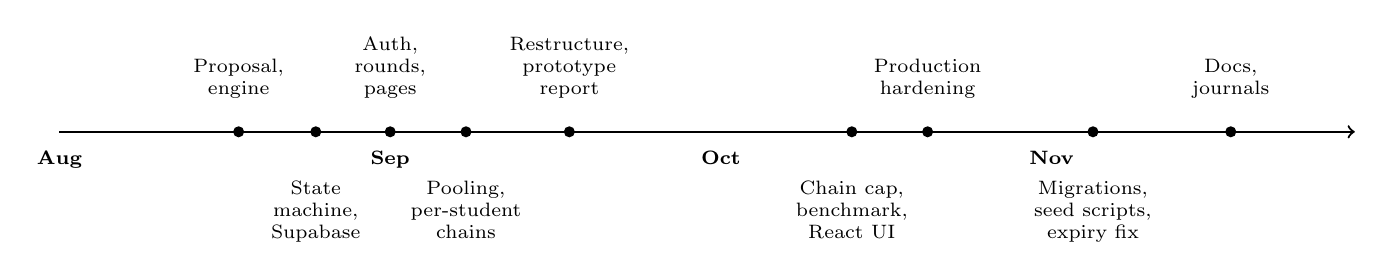
\begin{tikzpicture}[x=1.75cm]
  \draw[thick,->] (0,0) -- (9.4,0);
  \foreach \x/\m in {0/Aug, 2.4/Sep, 4.8/Oct, 7.2/Nov}
    \node[font=\scriptsize\bfseries, below] at (\x,-0.12) {\m};
  \foreach \x in {1.3,1.86,2.4,2.95,3.7,5.75,6.3,7.5,8.5}
    \fill (\x,0) circle (2pt);
  \node[font=\scriptsize, align=center, above=3mm] at (1.3,0) {Proposal,\\ engine};
  \node[font=\scriptsize, align=center, below=5mm] at (1.86,0) {State\\ machine,\\ Supabase};
  \node[font=\scriptsize, align=center, above=3mm] at (2.4,0) {Auth,\\ rounds,\\ pages};
  \node[font=\scriptsize, align=center, below=5mm] at (2.95,0) {Pooling,\\ per-student\\ chains};
  \node[font=\scriptsize, align=center, above=3mm] at (3.7,0) {Restructure,\\ prototype\\ report};
  \node[font=\scriptsize, align=center, below=5mm] at (5.75,0) {Chain cap,\\ benchmark,\\ React UI};
  \node[font=\scriptsize, align=center, above=3mm] at (6.3,0) {Production\\ hardening};
  \node[font=\scriptsize, align=center, below=5mm] at (7.5,0) {Migrations,\\ seed scripts,\\ expiry fix};
  \node[font=\scriptsize, align=center, above=3mm] at (8.5,0) {Docs,\\ journals};
\end{tikzpicture}}
\caption{Project timeline, August--November 2026}
\label{fig:timeline}
\end{figure}

The work fell into five phases:

\begin{enumerate}
  \item \textbf{Proposal and core engine (17--24 Aug).} Preference model,
  scoring, Hungarian and Murty matching, cycle extraction, the fairness
  filter, ranking, synthetic pools, scenario tests and CI; the approval
  state machine and the Supabase integration.
  \item \textbf{Authentication, rounds and pages (31 Aug).} Session
  authentication and roles, the round workflow in \texttt{rounds.py}, and
  the first student and admin pages.
  \item \textbf{Prototype stage (5--17 Sep).} Connection pooling, query
  optimisation, chains offered per student, the move of the package under
  \texttt{code/}, and the prototype report.
  \item \textbf{Chain cap, new UI and hardening (12 Oct -- 2 Nov).} The
  chain-length cap and its benchmark, the React interface with roommate
  requests, secure cookies, a fail-fast check for production, numbered
  migrations and seed scripts.
  \item \textbf{Expiry and documentation (3--16 Nov).} A review of the
  approval workflow found that proposals never expired and that settled
  chains kept their members locked out; both were fixed
  (Section~\ref{sec:expiry-defect}). The documentation site and weekly
  journals were brought up to date.
\end{enumerate}

Each member kept a weekly journal in the problem, cause and fix format,
published on the documentation site. Design decisions are recorded in the
code where they are made, next to the constant or check they justify,
so that the reason travels with the code (Section~\ref{sec:decisions}).

\section{Team Roles}

\begin{table}[H]
\centering
\small
\begin{tabularx}{\textwidth}{>{\raggedright\arraybackslash}p{0.22\textwidth} r L}
\toprule
\textbf{Member} & \textbf{Commits} & \textbf{Main areas} \\
\midrule
Aabhas Khandelwal & 17 & Matching engine, approval state machine, round workflow, proposal expiry, test suite, CI, reports \\
Aakash Chawla & 25 & Database layer, authentication, API, React interface, chain cap and benchmark, migrations, seed scripts \\
Joy Soni & 4 & First student and admin pages, secure session cookies \\
\bottomrule
\end{tabularx}
\caption{Team roles (non-merge commits on \texttt{development}, 17 Aug -- 16 Nov 2026)}
\label{tab:roles}
\end{table}

Commit counts show the recorded author only. Pair work, design discussion
and review are not visible in them, so they are a lower bound on each
member's contribution.
